\documentclass[11pt]{article}

\usepackage{fullpage}
\usepackage{url}
\usepackage{paralist}
\usepackage{graphicx}
\usepackage[small]{caption}
\usepackage{subfig}
\usepackage{multirow}

% =========
\usepackage{color}

% The xxx tag is intended to denote urgent text that needs addressing.
% The meh tag is intended to highlight text that needs some loving or which
% we're not sure should make primetime
\newcommand{\xxx}[1]{{\bf \color{red} #1}}
\newcommand{\meh}[1]{{\bf \color{blue} #1}}
\newcommand\T{\rule{0pt}{3ex}}
\newcommand\B{\rule[-1.2ex]{0pt}{0pt}}

% =========

\title{\xxx{Linguistic Classification of Objects}}
\author{Rob Goeddel \and Lauren Hinkle \and James Kirk \and Aaron Mininger}
\date{}

\begin{document}
\maketitle

\begin{abstract}
\xxx{Abstract goes here, 1 par. max}
Dijkstra was a cool guy and it's fun to cite his papers~\cite{dijkstra1959}. (It's true)
\end{abstract}

\section{Introduction}
\xxx{Problem description and motivation. Why do you want to solve this
    problem? What's the impact if you can solve this problem?}
Language is a powerful tool that is just coming into its own as the human
interface for various systems. Apple's Siri is an excellent example of this,
making interaction with your phone intuitive, easy, and efficient. 

Robotic systems in AI can also benefit from greater understanding of
language. Such knowledge could allow a human to command or teach a robot agent in a more natural way. Take, for example, a robotic arm system with knowledge of only
several nouns and actions: cup, sink, grab/move object, and turning on/off
the sink, and the spatial concept of in. Through language, the robot could then be taught the new action of ``filling a cup'', which means to put the cup in the sink and turn on the
sink. Even though the robot has never seen anyone fill a cup before, now
it should be able to do so itself. Furthermore, the agent could generalize the concept to new items, like a bowl. This is a powerful
and intuitive way for humans to interact with a system, one which does not
take a computer scientist to understand.

Our goal is to leverage machine learning techniques in order to train a system to know a small vocabulary of nouns, adjectives,
and actions. As a proof of concept, we want to be able to play the children's
game ``I spy'' with a robotic arm. The arm's ``eyes'' will be a Microsoft
Kinect (or, with some small probability, a stereo camera rig) capable of
returning RGB-D data for classification. A collection of objects will be placed in the view of the camera, and a person will give a description of one of the objects. The agent will then select the object that matches that description using the robot arm. \meh{Pointing? Grabbing?}.

This work is planned to be incorporated into a larger project which includes teaching the agent new concepts and actions as described above. Such a project relies on having symbolic information provided by our work through object segmentation and classification. The low level features provided by our system can be analyzed and combined in order to build new concepts like object categories (like blocks and balls) or object properties (all bananas are yellow). Such a system could be used on service tasks or with non-robotic systems where a verbal interface
offers improvements in efficiency, safety, etc. \xxx{Examples?}

\section{Proposed Method}
\xxx{How are you going to solve this problem? Why should the proposed method
    work? Provide technical details of your approach if you are proposing a
    novel method.}

Our approach will use supervised learning techniques to generate a description of each object. First, we will gather our training data by collecting a number of RGB-D images from the camera featuring various types and positions of objects. Each image will be run through a segmentation process to isolate every object in the scene. Each object will be manually given a label describing its color, shape, and size. From these segmentations we will extract a useful feature vector for each attribute. We will have one SVM for each possible label, and train it using all of the objects with that label verses all of the objects without that label. \meh{Are we using a bunch of binary SVMs or a multiclass?}

For object identification we will do a similar process to segment each object in the camera's image. That object's position in 3D space will be determined using both the pixel coordinate and the depth value. The features will then be extracted and run through our SVM's using the models created with the training data. This will give us a bag of words description for each object in the scene. This description, along with the position, will be given as input to a Soar agent. Soar is a cognitive architecture that will be responsible for the high-level reasoning and language processing. Our Soar agent will interpret the commands given by the users, determine which object is being described, and give the appropriate commands to the robotic arm. 

\xxx{What on EARTH do we say here, otherwise? One paragraph seems pretty
    thin. AM - I added a bit to this section, but we still might want to go into more detail}

\section{Related Work}
\xxx{What are existing methods? What are the state-of-the-art methods for this
    problem? How is your approach different from the related work?}

\section{Experimental Results}
\xxx{Milestones achieved so far (add all relevant experimental results). How
    do these results support your claim?}
\subsection{Infrastructure}
We have build/begun building several of the pieces necessary for our I-spy
game in parallel.  Prof. Edwin Olson has supplied the group with a robotic
arm (pictured in Figure~\ref{fig:arm}) and a Kinect, which we built an
overhead mount (pictured in Figure~\ref{fig:kinect-mount}) to allow it to view
a small (~2\,ft $\times$ 4\,ft) play area.

We calibrated the Kinect using an external package~\xxx{cite}, but may still
choose to calibrate it ourselves using several independent tools to see if we
can improve the calibration error. We are using the OpenKinect
package libfreenect~\cite{OpenKinect} to acquire data from the Kinect and have
written a small driver in C to output frames via LCM~\cite{huang2010} to simplify
communication with the driver for our Java code and because LCM offers useful
built-in logging capabilities.

\begin{figure}
\centering
\subfloat[Robotic arm \xxx{placeholder}] {
    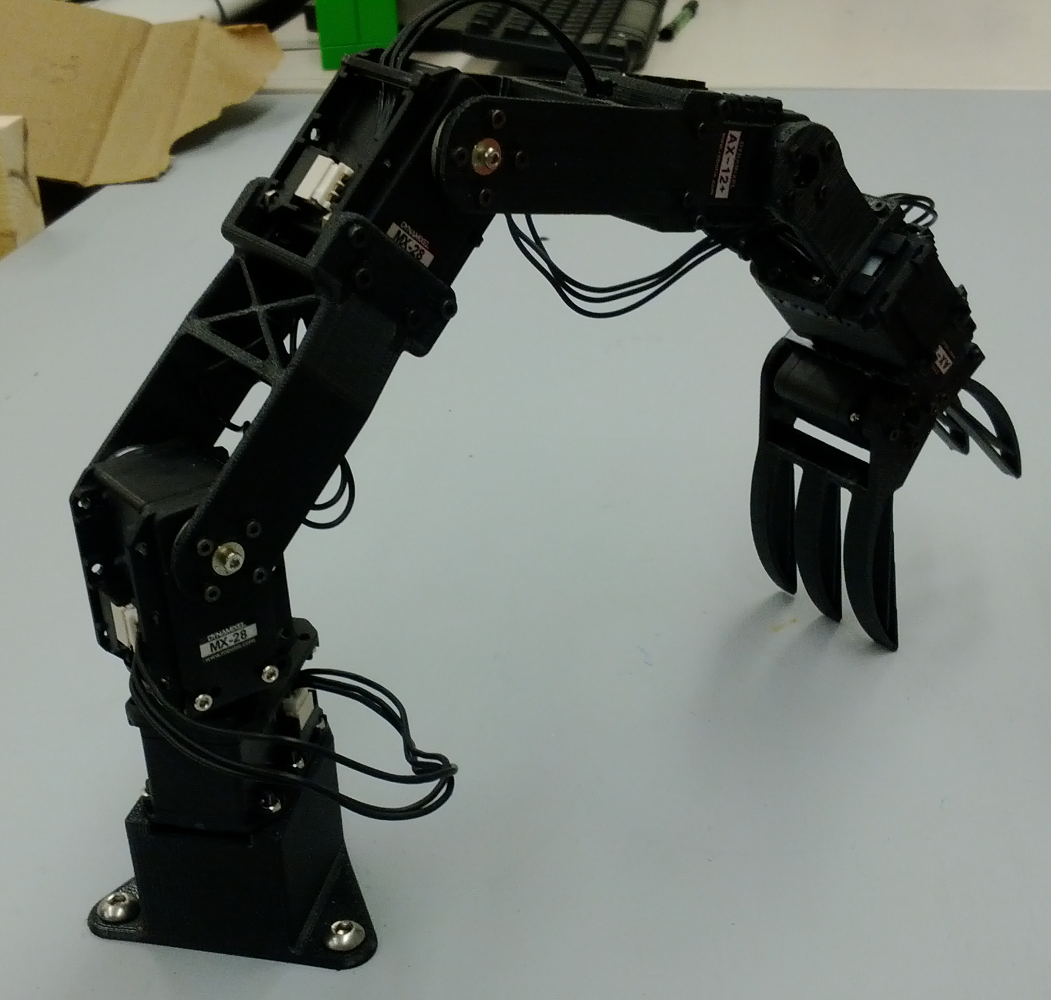
\includegraphics[height=3in]{figures/arm2.png}
    \label{fig:arm}
}
\subfloat[Kinect mount \xxx{placeholder}] {
    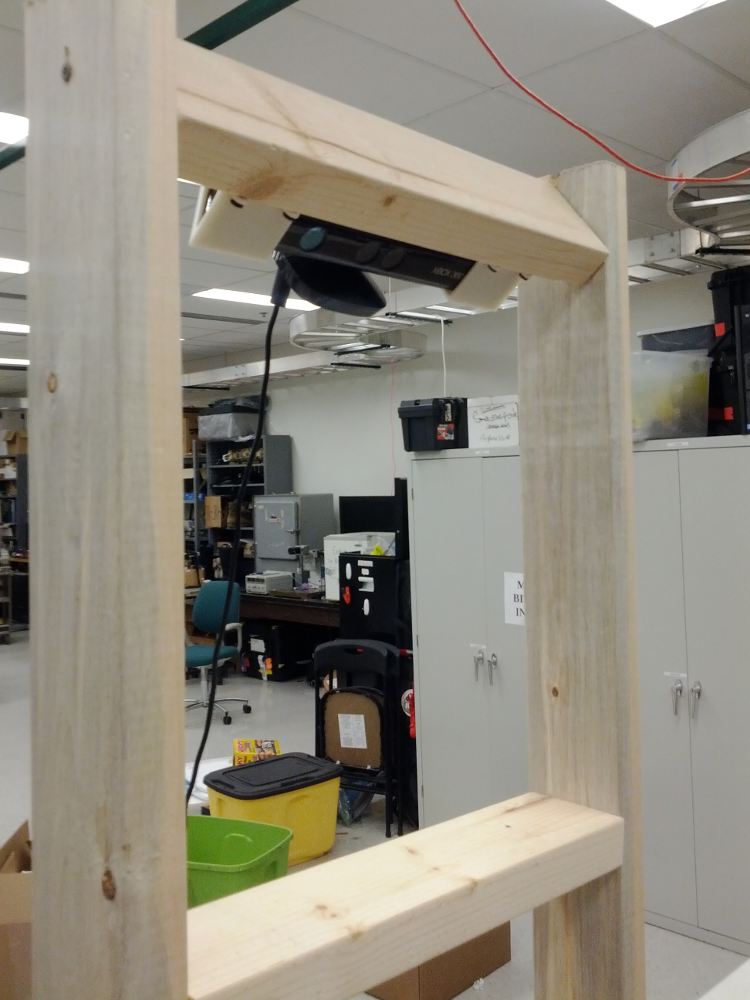
\includegraphics[height=3in]{figures/kinect.png}
    \label{fig:kinect-mount}
}
\caption{Our robotic arm and Kinect mount. \xxx{better caption}}
\label{fig:hardware}
\end{figure}

\subsection{Data Collection and Training}
We have acquired a large variety of children's foam blocks in many shapes and
colors to act as our objects for classification. A small subset of the blocks
can be seen in Figure~\ref{fig:blocks}. The foam the blocks is an ideal
material to work with as it
\begin{inparaenum}[(1)]
\item has a smooth, matte finish,
\item comes in a variety of distinct colors, and
\item is deformable enough to be grabbed by the arm but still retain its
shape.
\end{inparaenum}

We have collected a training dataset of footage of the foam blocks at numerous
positions and angles throughout the play area and are creating \xxx{have
created?} a tool that segments out objects from the scene and allows a human
to label these objects with relevant descriptors.

\xxx{More to come?}

\begin{figure}
\centering
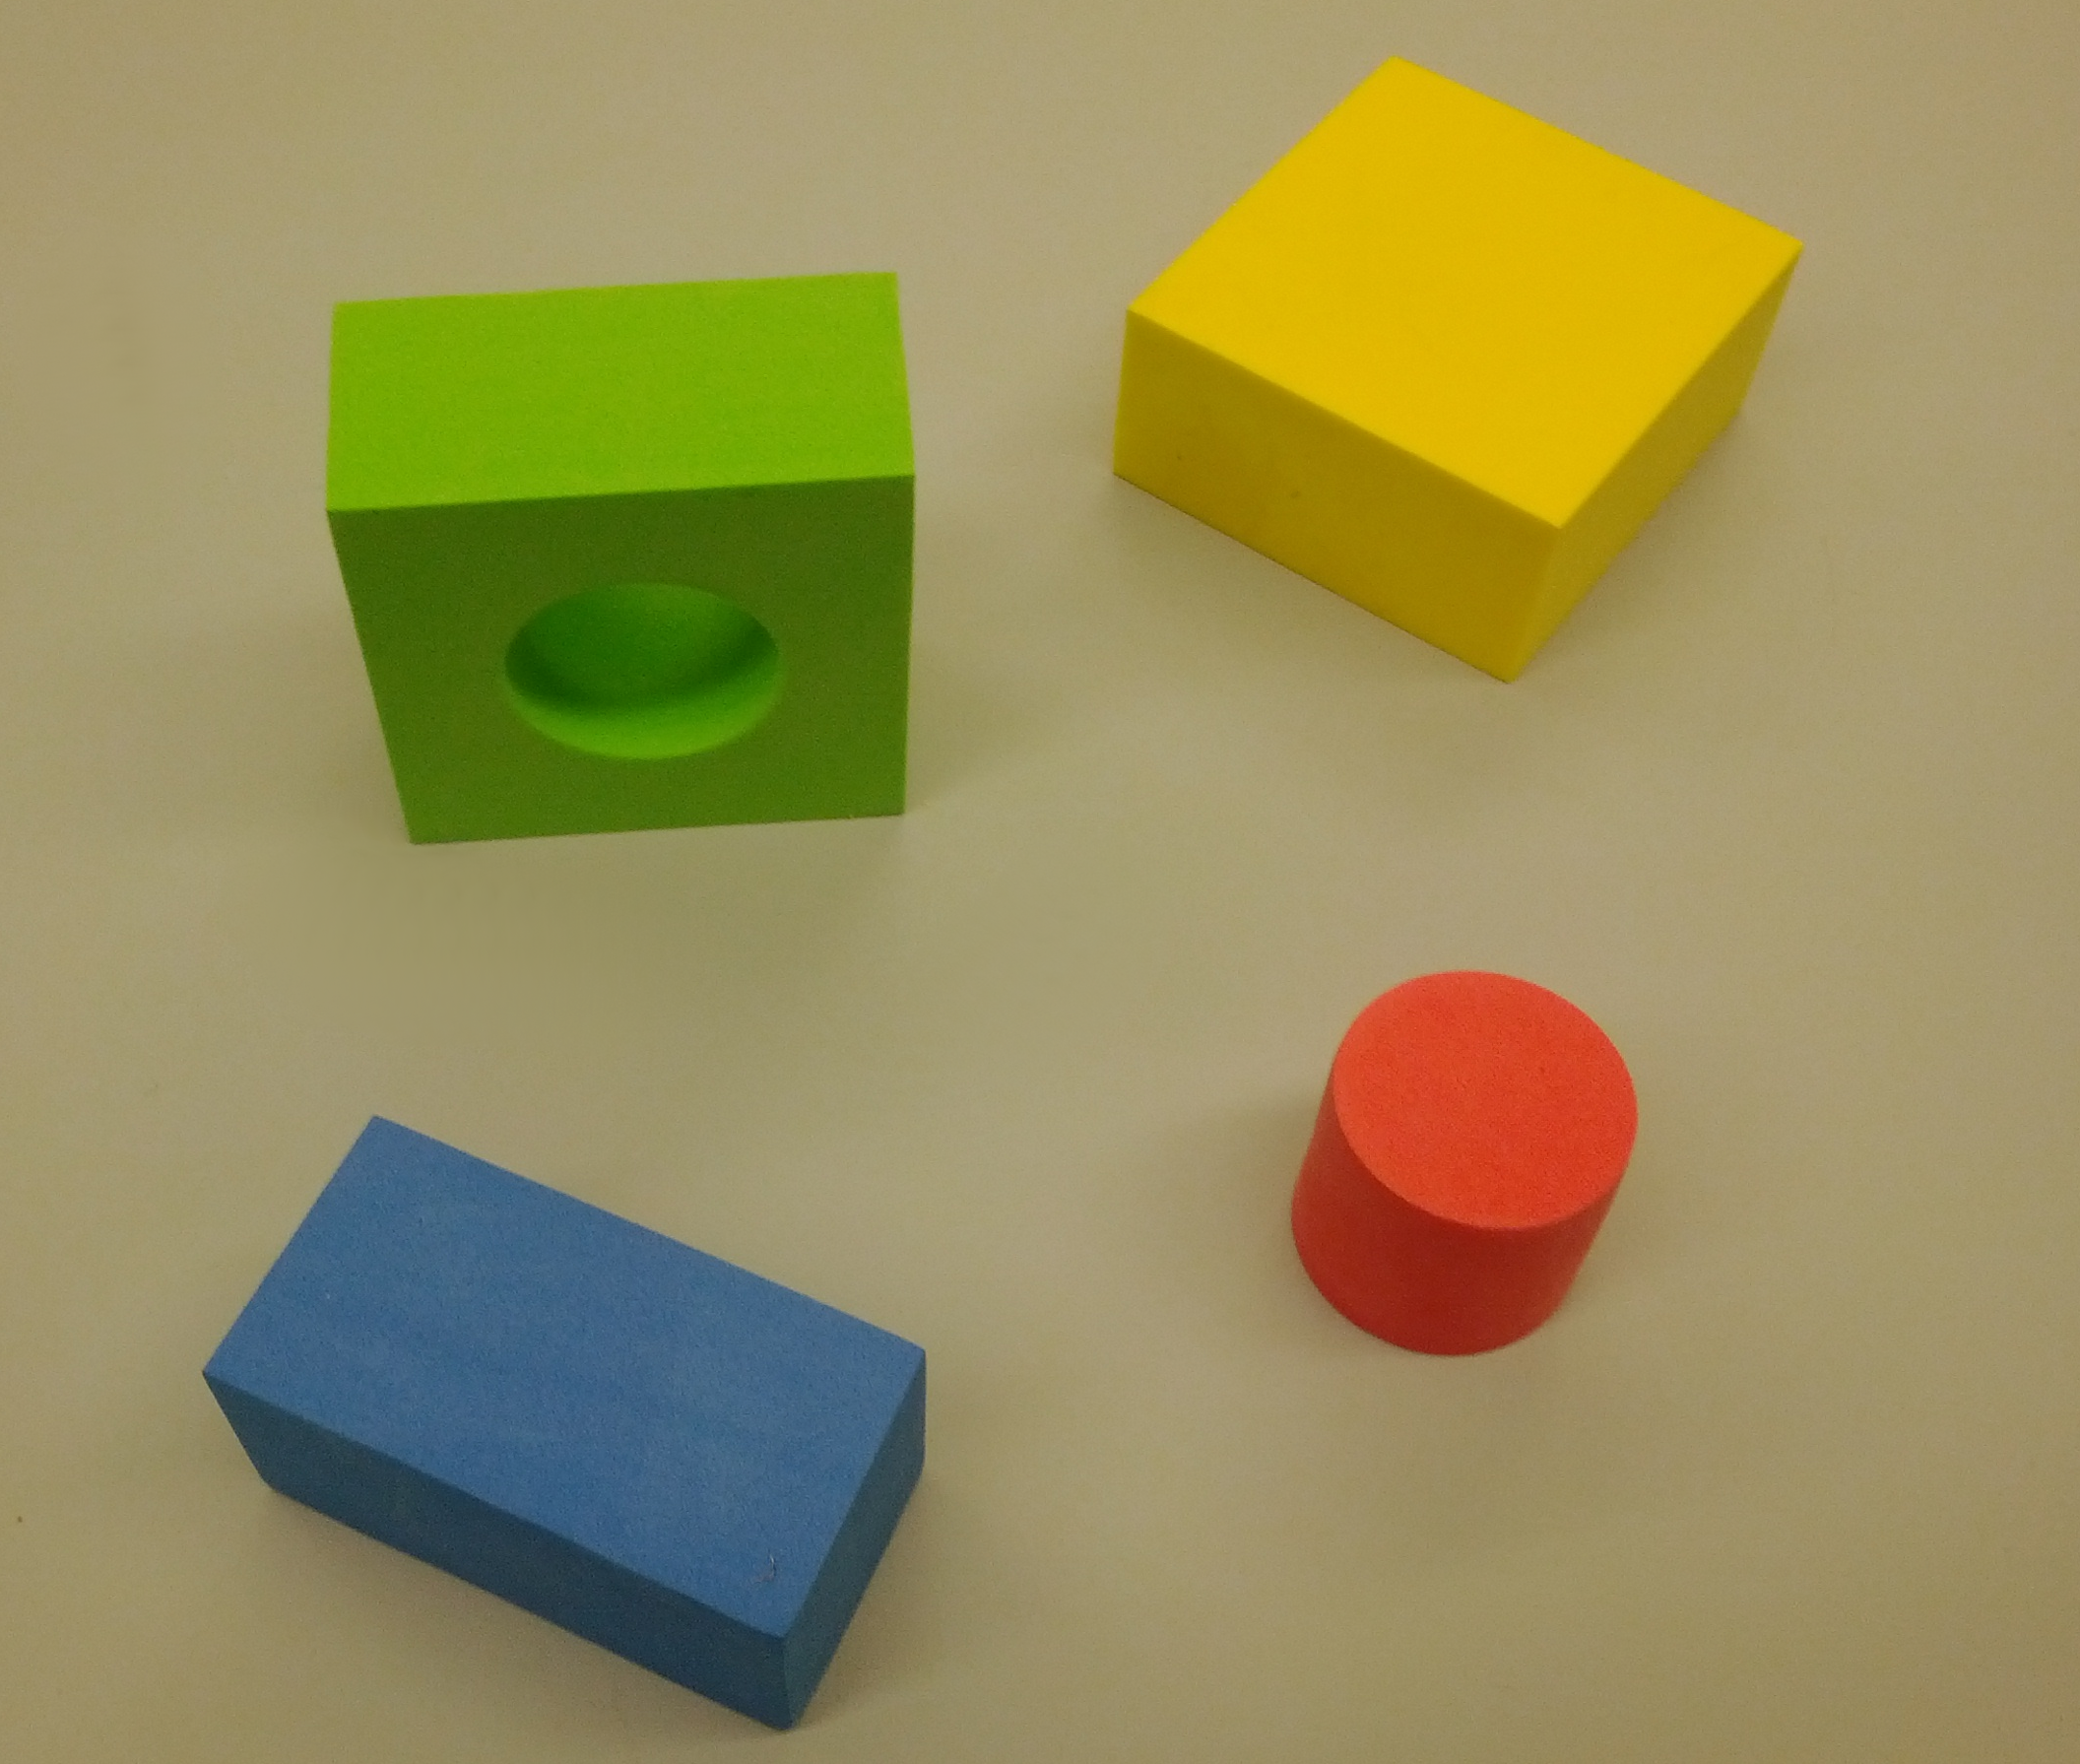
\includegraphics[width=0.48\textwidth]{figures/blocks.png}
\caption{A sample of the foam blocks we are using for classification. To
    simplify the language space we are working in, we limited our objects to
    those that can be described with simple shapes and colors.}
\label{fig:blocks}
\end{figure}

\section{Future Milestones}
\xxx{Dates and sub-goals (please set sub-goals on a weekly basis so that they
    can be done in a week)}

\meh{Due to a looming paper deadline on 10~Mar for Lauren and Rob, data
    processing for training purposes has taken a backseat to paper writing.
    Rapid progress is expected post-deadline when this additional workload
    disappears.}

\begin{center}
    \begin{tabular}{ | l | l |}
    \hline
    \multirow{2}{*}{11~Mar -- 17~Mar} 
	& Full labeling of the training data \T \\
	& SVM trained using the color features \B \\ 
    \hline
    \multirow{2}{*}{18~Mar -- 24~Mar} 
	& Evaluation and tuning of color classification \T \\ 
	& Object Localization (determining an object's position in 3D space) \B \\ 
    \hline
    \multirow{2}{*}{25~Mar -- 31~Mar} 
	& Focus our time on the Machine Learning midterm \T\\
	& Have all the components of our system connected together ('water through the pipes') \B \\ 
    \hline
    \multirow{2}{*}{1~Apr -- 7~Apr} 
	& Test and debug the first assembled version of the system \T \\
	& Add shape features and classification to the system \B\\ 
    \hline
    \multirow{2}{*}{8~Apr -- 14~Apr} 
	& \meh{Board says test object disambiguation. Not quite sure what that means} \T\\
	& Evaluation and tuning of our shape classification \B \\ 
    \hline
    \multirow{3}{*}{15~Apr -- 21~Apr} 
	& Implement the user interface, including the 'I Spy' game format \T\\
	& Full evaluation of the system \\ 
	& Start writing up the report and the poster \B \\
    \hline
    \multirow{3}{*}{21~Apr -- 24~Apr} 
	& Finish editing final report \T \\
	& Finish editing poster and print final copy \\ 
	& Prepare and practice the presentation \B \\
    \hline
    \end{tabular}
\end{center}

\section{Conclusion}
\xxx{Summary of your progress and your final expected goal (what do you expect
    to achieve or demonstrate for the final project?)}

\bibliographystyle{plain}
\bibliography{literature}

\end{document}
